\documentclass[tikz,border=5pt]{standalone}
\usepackage[UTF8]{ctex}
\usepackage{amsmath,amssymb}
\usetikzlibrary{arrows.meta,calc,angles,quotes}
\tikzset{>=Stealth,line cap=round,line join=round,
aux/.style={gray!55,dashed,thin},
dim/.style={gray!70,<->,thin},
ropeA/.style={red!65!black,very thick},
ropeB/.style={blue!65!black,very thick}}
\newcommand{\cone}[2]{
\pgfmathsetmacro{\coneTheta}{#1}
\pgfmathsetmacro{\coneHeight}{#2}
\pgfmathsetmacro{\rim}{asin(.32*tan(\coneTheta)/.9474)}
\draw[gray!65,dashed,thin]plot[domain=\rim:180-\rim,samples=61]
({\coneHeight*sin(\coneTheta)*cos(\x)},{\coneHeight*sin(\coneTheta)*sin(\x)},{-\coneHeight*cos(\coneTheta)});
\draw[gray!65,thin]plot[domain=180-\rim:360+\rim,samples=81]
({\coneHeight*sin(\coneTheta)*cos(\x)},{\coneHeight*sin(\coneTheta)*sin(\x)},{-\coneHeight*cos(\coneTheta)});
\draw[gray!70] (0,0,0)--({\coneHeight*sin(\coneTheta)*cos(\rim)},{\coneHeight*sin(\coneTheta)*sin(\rim)},{-\coneHeight*cos(\coneTheta)});
\draw[gray!70] (0,0,0)--({\coneHeight*sin(\coneTheta)*cos(180-\rim)},{\coneHeight*sin(\coneTheta)*sin(180-\rim)},{-\coneHeight*cos(\coneTheta)});
\node[above]at(0,0,0){$O$};
}
\begin{document}
% 1. Real cone geodesics: r cos[sin(theta)(phi-mid)] is constant.
\begin{tikzpicture}[font=\small,
x={(1cm,0cm)},y={(0cm,.32cm)},z={(0cm,.9474cm)}]
\begin{scope}
\cone{30}{5.4}
\pgfmathsetmacro{\rzero}{3.2}
\pgfmathsetmacro{\cut}{asin(.32*tan(30)/.9474)}
\draw[ropeB]plot[domain=-60:\cut,samples=61,variable=\p]
({\rzero*cos(45)/cos(.5*(\p-30))*sin(30)*cos(\p)},
{\rzero*cos(45)/cos(.5*(\p-30))*sin(30)*sin(\p)},
{-\rzero*cos(45)/cos(.5*(\p-30))*cos(30)});
\draw[ropeB,dashed]plot[domain=\cut:120,samples=61,variable=\p]
({\rzero*cos(45)/cos(.5*(\p-30))*sin(30)*cos(\p)},
{\rzero*cos(45)/cos(.5*(\p-30))*sin(30)*sin(\p)},
{-\rzero*cos(45)/cos(.5*(\p-30))*cos(30)});
\draw[ropeB,dashed]plot[domain=120:180-\cut,samples=51,variable=\p]
({\rzero*cos(45)/cos(.5*(\p-210))*sin(30)*cos(\p)},
{\rzero*cos(45)/cos(.5*(\p-210))*sin(30)*sin(\p)},
{-\rzero*cos(45)/cos(.5*(\p-210))*cos(30)});
\draw[ropeB]plot[domain=180-\cut:300,samples=61,variable=\p]
({\rzero*cos(45)/cos(.5*(\p-210))*sin(30)*cos(\p)},
{\rzero*cos(45)/cos(.5*(\p-210))*sin(30)*sin(\p)},
{-\rzero*cos(45)/cos(.5*(\p-210))*cos(30)});
\coordinate(A)at({3.2*.5*cos(-60)},{3.2*.5*sin(-60)},{-3.2*cos(30)});
\coordinate(B)at({3.2*.5*cos(120)},{3.2*.5*sin(120)},{-3.2*cos(30)});
\filldraw[fill=white,thick](A)circle(2.5pt);
\draw[dashed,fill=white,thick](B)circle(2.5pt);
\node[below right,fill=white,inner sep=1pt]at(A){$A\ (m)$};
\node[above left,xshift=-10pt,yshift=10pt,inner sep=1pt]at(B){$B\ (m)$};
\node at(0,0,-6.0){绳套连接};
\end{scope}
\begin{scope}[xshift=7cm]
\cone{19.4712206345}{5.4}
\pgfmathsetmacro{\coneTheta}{19.4712206345}
\pgfmathsetmacro{\rzero}{2.9}
\pgfmathsetmacro{\cut}{asin(.32*tan(\coneTheta)/.9474)}
\draw[ropeB]plot[domain=-60:\cut,samples=61,variable=\p]
({\rzero*cos(30)/cos((\p-30)/3)*sin(\coneTheta)*cos(\p)},
{\rzero*cos(30)/cos((\p-30)/3)*sin(\coneTheta)*sin(\p)},
{-\rzero*cos(30)/cos((\p-30)/3)*cos(\coneTheta)});
\draw[ropeB,dashed]plot[domain=\cut:120,samples=61,variable=\p]
({\rzero*cos(30)/cos((\p-30)/3)*sin(\coneTheta)*cos(\p)},
{\rzero*cos(30)/cos((\p-30)/3)*sin(\coneTheta)*sin(\p)},
{-\rzero*cos(30)/cos((\p-30)/3)*cos(\coneTheta)});
\draw[ropeA,dashed]plot[domain=120:180-\cut,samples=61,variable=\p]
({\rzero*cos(30)/cos((\p-210)/3)*sin(\coneTheta)*cos(\p)},
{\rzero*cos(30)/cos((\p-210)/3)*sin(\coneTheta)*sin(\p)},
{-\rzero*cos(30)/cos((\p-210)/3)*cos(\coneTheta)});
\draw[ropeA]plot[domain=180-\cut:300,samples=61,variable=\p]
({\rzero*cos(30)/cos((\p-210)/3)*sin(\coneTheta)*cos(\p)},
{\rzero*cos(30)/cos((\p-210)/3)*sin(\coneTheta)*sin(\p)},
{-\rzero*cos(30)/cos((\p-210)/3)*cos(\coneTheta)});
\coordinate(P)at({2.9/3*cos(-60)},{2.9/3*sin(-60)},{-2.9*cos(\coneTheta)});
\coordinate(Q)at({2.9/3*cos(120)},{2.9/3*sin(120)},{-2.9*cos(\coneTheta)});
\coordinate(A2)at({4/3*cos(-60)},{4/3*sin(-60)},{-4*cos(\coneTheta)});
\coordinate(B2)at({4.8/3*cos(120)},{4.8/3*sin(120)},{-4.8*cos(\coneTheta)});
\draw[ropeA](P)--(A2);
\draw[ropeB,dashed](Q)--(B2);
\filldraw[fill=white,thick](P)circle(2.5pt);
\draw[fill=white,dashed,thick](Q)circle(2.5pt);
\node[right,fill=white,inner sep=1pt]at(P){$P$};
\node[above left,xshift=-8pt,yshift=8pt,inner sep=1pt]at(Q){$Q$};
\filldraw[fill=white,thick](A2)circle(3pt);
\draw[fill=white,dashed,thick](B2)circle(3pt);
\node[right,fill=white,inner sep=1pt]at(A2){$A\ (m)$};
\node[left,fill=white,inner sep=1pt]at(B2){$B\ (m)$};
\node at(0,0,-6.0){交叉过环连接};
\end{scope}
\node[black!70]at(3.5,0,-6.65){虚线表示背侧遮挡；末段绳贴着母线};
\end{tikzpicture}
% 2. Actual meridional section and isometric half-sector, not a spatial chord.
\begin{tikzpicture}[font=\small]
\begin{scope}
\coordinate(O)at(0,3.8);\coordinate(C)at(0,0);
\coordinate(P)at(2.1,0);
\draw[gray!70,thick](O)--(P);
\draw[aux](O)--(C);
\draw[dim](0,-.25)--(2.1,-.25)node[midway,below]{$R=x\sin\theta$};
\node[left]at(O){$O$};\node[left]at(C){$C$};\node[right]at(P){$P$};
\draw[dim](-.5,3.8)--(-.5,0)node[midway,left]{$x\cos\theta$};
\node[above right]at(1.05,1.9){$x$};
\pic[draw,angle radius=.70cm,"$\theta$",angle eccentricity=1.4]{angle=C--O--P};
\draw[aux](C)--(P);
\node at(1,-1){母线截面};
\end{scope}
\begin{scope}[xshift=7.1cm,yshift=3.8cm]
\coordinate(V)at(0,0);
\coordinate(P)at(-2.2,-3.8105);\coordinate(Q)at(2.2,-3.8105);
\draw[gray!70](V)--(P);\draw[gray!70](V)--(Q);
\draw[gray!60,dashed](-2.2,-3.8105)arc[start angle=240,end angle=300,radius=4.4];
\draw[ropeB](P)--(Q);
\draw[aux](V)--(0,-3.8105);
\node[above]at(V){$O$};\node[below left]at(P){$P$};
\node[below right]at(Q){$Q$};
\node[left]at(-1.15,-1.9){$x$};\node[right]at(1.15,-1.9){$x$};
\node[above]at(0,-3.8105){$d=2x\sin\beta$};
\draw(-.55,-.9526)arc[start angle=240,end angle=300,radius=1.1];
\node[fill=white,inner sep=1pt]at(0,-1.27){$\alpha=2\beta$};
\node[right,fill=white,inner sep=1pt]at(.05,-2.60){$x\cos\beta$};
\node at(0,-4.55){$\alpha=\pi\sin\theta$};
\node at(0,-4.95){半圈锥面等距展开};
\end{scope}
\end{tikzpicture}
% 3. Tangent-plane sum and genuine gravity/normal decomposition, separate panels.
\begin{tikzpicture}[font=\small]
\begin{scope}
\fill(0,0)circle(2pt);
\draw[aux](0,-1.55)--(0,1.65);
\draw[ropeB,->](0,0)--(-1.732,1)node[left]{$T$};
\draw[ropeB,->](0,0)--(1.732,1)node[right]{$T$};
\draw[blue!65!black,->,thick](0,0)--(0,1.65)node[above]{$2T\sin\beta$};
\draw[red!65!black,->,thick](0,0)--(0,-1.2)node[below]{$mg\cos\theta$};
\draw[gray!65,->](-.5,-.45)--(.8,-.45)node[right]{$\boldsymbol e_\varphi$};
\node[left]at(0,-.85){$\boldsymbol e_r$};
\draw(-.52,.30)arc[start angle=150,end angle=90,radius=.60];
\node at(-.48,.72){$\frac{\pi}{2}-\beta$};
\node at(0,-2.55){切平面内的投影};
\end{scope}
\begin{scope}[xshift=6.8cm,yshift=.5cm]
\coordinate(W)at(0,0);
\draw[gray!50](-1.5,2.6)--(1.35,-2.338);
\fill(W)circle(2pt);
\draw[red!65!black,->,thick](W)--(0,-2.2)node[below]{$mg$};
\draw[blue!65!black,->,thick](W)--(.9526,.55)node[above right]{$N$};
\draw[gray!65,dashed,->](W)--(.9526,-1.65)node[right]{$mg\cos\theta$};
\draw[gray!65,dashed,->](W)--(-.9526,-.55)node[left]{$mg\sin\theta$};
\draw[aux](.9526,-1.65)--(0,-2.2);
\draw[aux](-.9526,-.55)--(0,-2.2);
\draw[gray!65,->](1.1,-1.30)--(1.6,-2.166)node[right]{$\boldsymbol e_r$};
\draw(0,-.6)arc[start angle=270,end angle=300,radius=.6];
\node at(.31,-.80){$\theta$};
\node at(.25,-3.05){重力与法向支承};
\end{scope}
\end{tikzpicture}
% 4. Connection order schematic, and a local free ring (no weight added).
\begin{tikzpicture}[font=\small]
\begin{scope}
\coordinate(P)at(0,0);\coordinate(Q)at(4.0,0);
\draw[ropeB](P)to[out=50,in=130](Q)to[out=-50,in=90](4.7,-1.65);
\draw[ropeA](Q)to[out=220,in=-40](P)to[out=220,in=90](-.7,-1.65);
\draw[fill=white,thick](P)circle(.09);
\draw[fill=white,thick](Q)circle(.09);
\fill[blue!65!black](.045,.07)circle(1.4pt);
\fill[red!65!black](3.945,-.065)circle(1.4pt);
\node[left]at(P){$P$};\node[right]at(Q){$Q$};
\node[blue!65!black,above]at(2,1){绳 $B:\ T_B$};
\node[red!65!black,below]at(2,-1){绳 $A:\ T_A$};
\draw[fill=white](-.7,-1.65)circle(.11);
\draw[fill=white](4.7,-1.65)circle(.11);
\node[below]at(-.7,-1.76){$A\ (m)$};
\node[below]at(4.7,-1.76){$B\ (m)$};
\node[gray!70]at(2,-2.55){连接顺序示意，不表示空间几何};
\node[gray!70]at(2,-3.00){小实点为固定端；空心环为穿绳处};
\end{scope}
\begin{scope}[xshift=8cm]
\draw[fill=white,thick](0,0)circle(.095);
\draw[ropeA,->](-.05,.075)--(-1.65,.998)node[left]{$T_A$};
\draw[ropeB,->](.05,.075)--(1.65,.998)node[right]{$T_B$};
\draw[ropeA,->](0,-.095)--(0,-1.60)node[below]{$T_A$};
\draw[aux](0,.10)--(0,1.55);
\node[above]at(0,1.55){上行母线};
\node[left]at(-.12,-.15){$P$};
\draw(-.433,.25)arc[start angle=150,end angle=90,radius=.5];
\node at(-.43,.63){$\frac{\pi}{2}-\beta$};
\node at(0,-2.55){轻环 $P$ 的三股绳力};
\end{scope}
\end{tikzpicture}
% 5. Unequal endpoints: same angle alpha, different radial distances a,b.
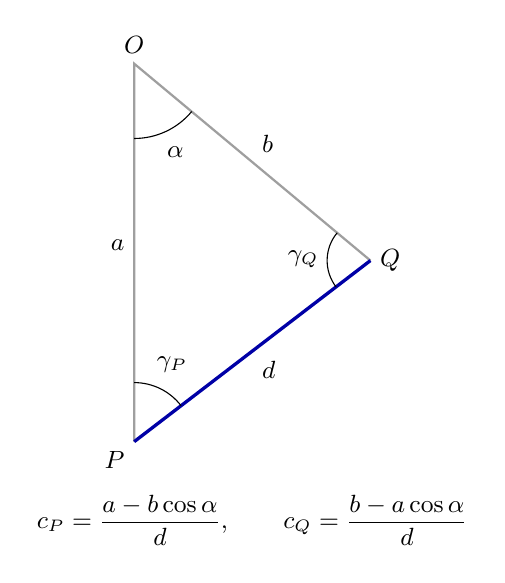
\begin{tikzpicture}[font=\small]
\coordinate(O)at(0,4.8);\coordinate(P)at(0,0);\coordinate(Q)at(3,2.3);
\draw[gray!75,thick](P)--(O)--(Q);
\draw[ropeB](P)--(Q);
\node[above]at(O){$O$};\node[below left]at(P){$P$};
\node[right]at(Q){$Q$};
\node[left]at(0,2.5){$a$};
\node[above right]at(1.5,3.55){$b$};
\node[below right]at(1.5,1.15){$d$};
\pic[draw,angle radius=.95cm,"$\alpha$",angle eccentricity=1.30]{angle=P--O--Q};
\pic[draw,angle radius=.75cm,"$\gamma_P$",angle eccentricity=1.45]{angle=Q--P--O};
\pic[draw,angle radius=.55cm,"$\gamma_Q$",angle eccentricity=1.55]{angle=O--Q--P};
\node[align=center]at(1.5,-1.0){
$c_P=\dfrac{a-b\cos\alpha}{d},\qquad
c_Q=\dfrac{b-a\cos\alpha}{d}$};
\end{tikzpicture}
\end{document}
